\documentclass[12pt]{article}
\usepackage{amsmath, amssymb, amsthm}
\usepackage{mathtools}
\usepackage{graphicx}
\usepackage{float}
\usepackage{hyperref}
\usepackage{xcolor}
\usepackage{listings}
\usepackage{geometry}
\usepackage{algorithm}
\usepackage{algpseudocode}
\usepackage{tikz}
\usepackage{longtable}
\usepackage{circuitikz}
\usepackage{comment}
\usepackage[section]{placeins}

% Page Setup
\geometry{a4paper, margin=1in}
\setlength{\intextsep}{10pt} % Space between text and floats
\bibliographystyle{IEEEtran}

% Custom Commands
\newcommand{\vecb}[1]{\mathbf{#1}}
\newcommand{\brak}[1]{\ensuremath{\left(#1\right)}}
\newcommand{\cbrak}[1]{\ensuremath{\left\{#1\right\}}}
\newcommand{\abs}[1]{\left\vert#1\right\vert}
\newcommand{\norm}[1]{\left\lVert#1\right\rVert}

\begin{document}
\title{}
\author{}
%{\let\newpage\relax\maketitle}
\section{Stability and error analysis}
\subsection{Forward Euler Method}
The update equation for forward euler's method is given by,
\begin{align*}
i_{n+1} &= i_n + hf(t_n, i_n) \\
        &= i_n + \frac{h}{L} \left[ V_{\text{in}}(t_n) - i_n R \right] \\
        &= i_n \left( 1 - \frac{R h}{L} \right) + \frac{h}{L} V_{\text{in}}(t_n)\\
        \text{Growth Factor } &= 1 - \frac{R h}{L}
\end{align*}

For the numerical solution to be stable,
\begin{align*}
        \implies \left| 1 - \frac{R h}{L} \right| &< 1 \\
        -1 &< 1 - \frac{R h}{L} < 1 \\
        \implies \frac{R}{L} &< \frac{2}{h}
\end{align*}

For the purpose of this analysis, we take $R = 1000, 1500, 1750, 2000, 2100$, $L = 0.001$ and step size $\brak{h} = 10^{-6}$.\newline
Stability is achieved when,
\begin{align*}
    \frac{R}{L} &< 2\times10^6\\
    \implies R &< 2000
\end{align*}

\textbf{Local Truncation Error}: The local truncation error for Forward Euler is $O(h^2)$. This represents the error introduced in a single step, assuming the previous value is exact. It can be derived from Taylor series expansion of the exact solution.

\textbf{Global Truncation Error}: The global truncation error for Forward Euler is $O(h)$. This accumulated error is one order lower than the local error because errors propagate and compound through each iteration of the numerical solution.

\textbf{Error Characteristics}:
\begin{itemize}
    \item First-order convergence (halving step size only reduces error by factor of 2).
    \item Highly sensitive to stiff problems.
    \item No numerical damping, tends to overshoot.
\end{itemize}

The plots clearly shows that at $R = 2000$, the system shows visible signs of instability. Whereas when $R$ exceeds $2000$, which in this case $R = 2100$, the system goes extremely unstable and the current blows up.
\newline

Another interesting point is that as the system is near instability, i.e. $R/L$ ratio is high, the response overshoots above normal response behaviour due to low numerical damping.

\begin{figure*}[!htb]
    {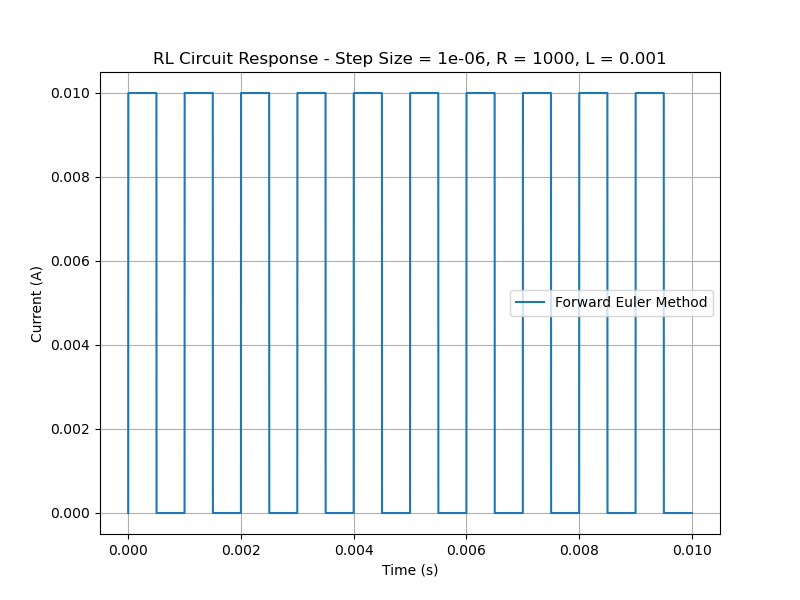
\includegraphics[ width=0.5\textwidth]{./figs/euler_R1000_L0.001.png}}
    \hspace{\fill}
    {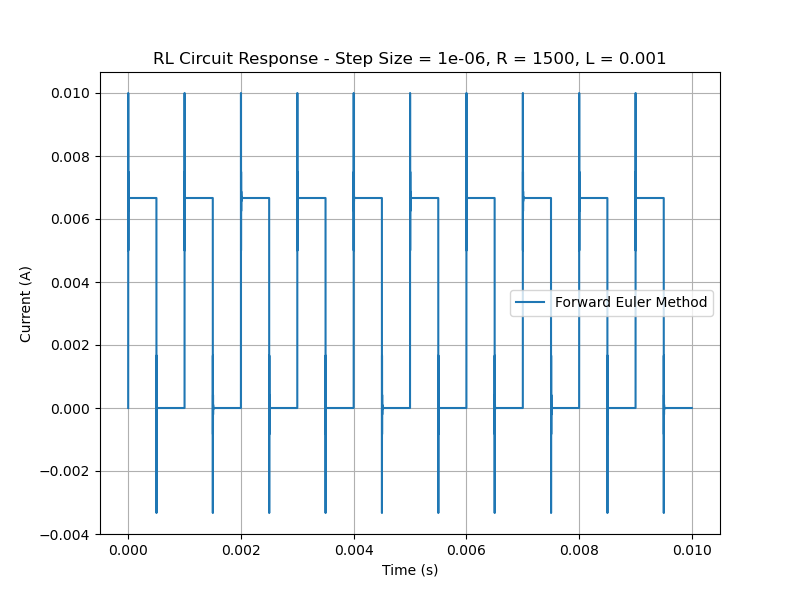
\includegraphics[ width=0.5\textwidth]{./figs/euler_R1500_L0.001.png}}
\end{figure*}
\begin{figure*}[!htb]
    {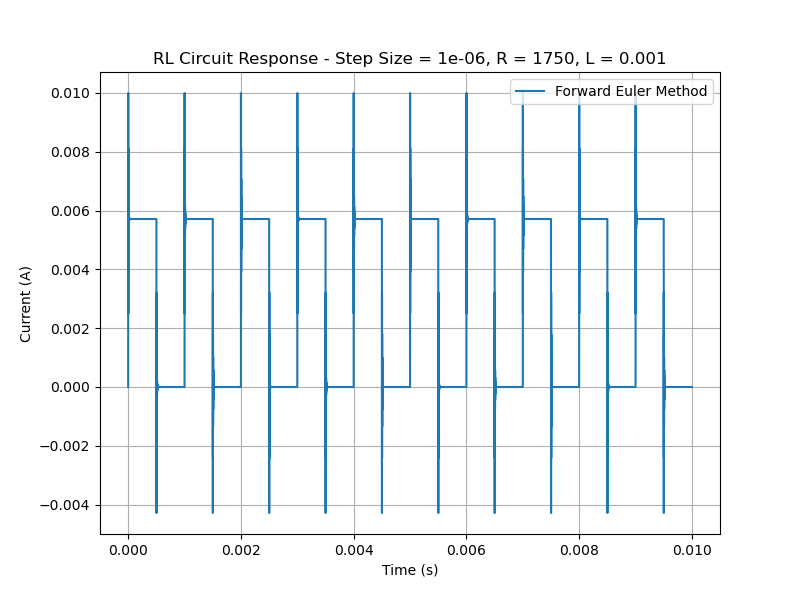
\includegraphics[ width=0.5\textwidth]{./figs/euler_R1750_L0.001.png}}
    \hspace{\fill}
    {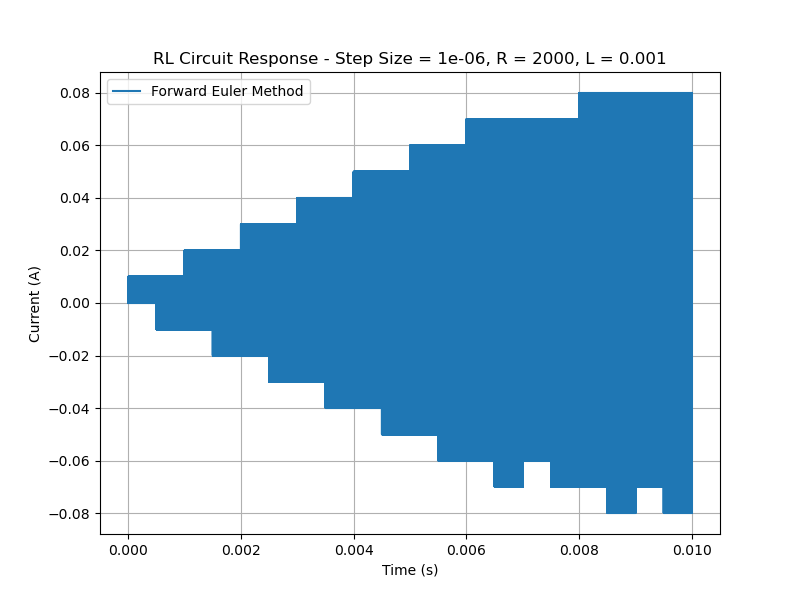
\includegraphics[ width=0.5\textwidth]{./figs/euler_R2000_L0.001.png}}
\end{figure*}
\begin{figure*}[!htb]
    {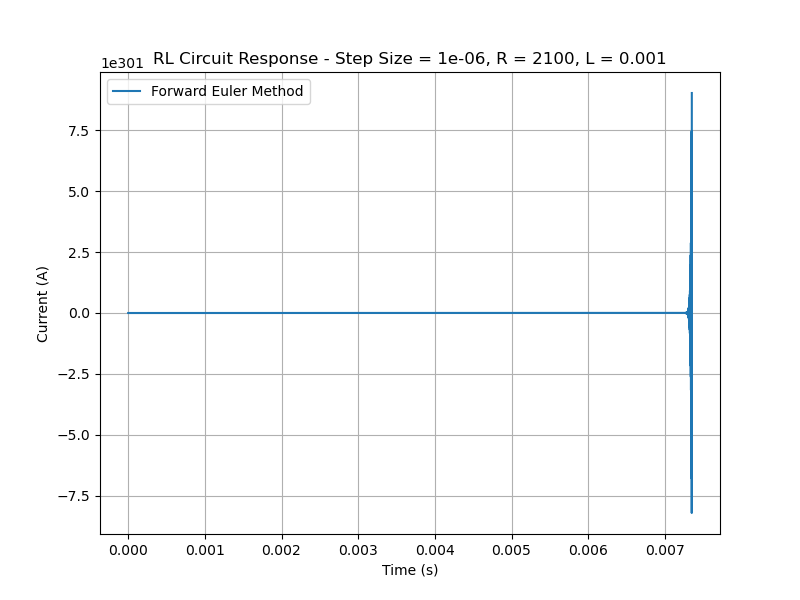
\includegraphics[ width=0.99\textwidth]{./figs/euler_R2100_L0.001.png}}
\end{figure*}


\subsection{RK2 Method}
The update equation for RK2 method is given by,
\begin{align*}
i_{n+1} &= i_n + \frac{h}{2} \Big[ f(t_n, i_n) + f(t_n + h, i_n + h f(t_n, i_n)) \Big] \\
i_{n+1} &= i_n + \frac{h}{2L} \Big[ V_{\text{in}}(t_n) - i_n R + V_{\text{in}}(t_n + h) - (i_n R) - \frac{h}{L} (V_{\text{in}}(t_n) - i_n)R \Big] \\
i_{n+1} &= i_n + \frac{h}{2L} \Big[ V_{\text{in}}(t_n) (1 - hR/L) - i_n (2R - Rh/L) + V_{in}\brak{t_n + h} \Big] \\
i_{n+1} &= i_n \left( 1 - \frac{R}{L}h + \brak{\frac{R}{L}}^2\frac{h^2}{2}\right) + \frac{h}{2L} V_{\text{in}}(t_n) (1 - hR/L) + \frac{h}{2L}V_{in}\brak{t_n + h}\\
\text{Growth Factor } &= 1 - \frac{R}{L}h + \brak{\frac{R}{L}}^2\frac{h^2}{2}
\end{align*}

Let $\frac{R}{L} = \alpha$. For the solution to be stable
\begin{align*}
\left| \frac{\alpha^2 h^2}{2} - \alpha h + 1 \right| < 1, \\
        -1 &< \frac{\alpha^2 h^2}{2} - \alpha h + 1 < 1, \\
        \frac{\alpha^2 h^2}{2} - \alpha h + 1 &< 1, \\
        \frac{\alpha^2 h^2}{2} - \alpha h &< 0, \\
        \Rightarrow \alpha h \left( \frac{\alpha h}{2} - 1 \right) &< 0, \\
        \Rightarrow \frac{R}{L} &< \frac{2}{h}, \\
\end{align*}
Also,
\begin{align*}
        \frac{\alpha^2 h^2}{2} - \alpha h + 2 &> 0, \\
        \alpha^2 h^2 - 2\alpha h + 4 &> 0, \\
        (\alpha h - 1)^2 + 3 &> 0.
\end{align*}
which is always true.

\textbf{Local Truncation Error}: The local truncation error for RK2 is $O(h^3)$. This improved accuracy comes from including second-order terms in the Taylor series expansion.

\textbf{Global Truncation Error}: The global truncation error for RK2 is $O(h^2)$. This second-order accuracy provides significantly better results than Forward Euler.

\textbf{Error Characteristics}:
\begin{itemize}
\item Second-order convergence (halving step size reduces error by factor of 4).
\item Better approximation near stability boundaries with less severe oscillations.
\end{itemize}

For the purpose of this analysis, we take $R = 1000, 1500, 1750, 2000, 2100$, $L = 0.001$ and step size $\brak{h} = 10^{-6}$.\newline
Stability is achieved when,
\begin{align*}
\frac{R}{L} &< \frac{2}{h}\\
\frac{R}{L} &< 2\times10^6\\
\implies R &< 2000
\end{align*}

The plots clearly shows that at $R = 2000$, the system shows visible signs of instability. Whereas when $R$ exceeds $2000$, which in this case $R = 2100$, the response goes extremely unstable and the current blows up. This behaviour is same as that observed in Forward Euler method.

\begin{figure*}[!htb]
{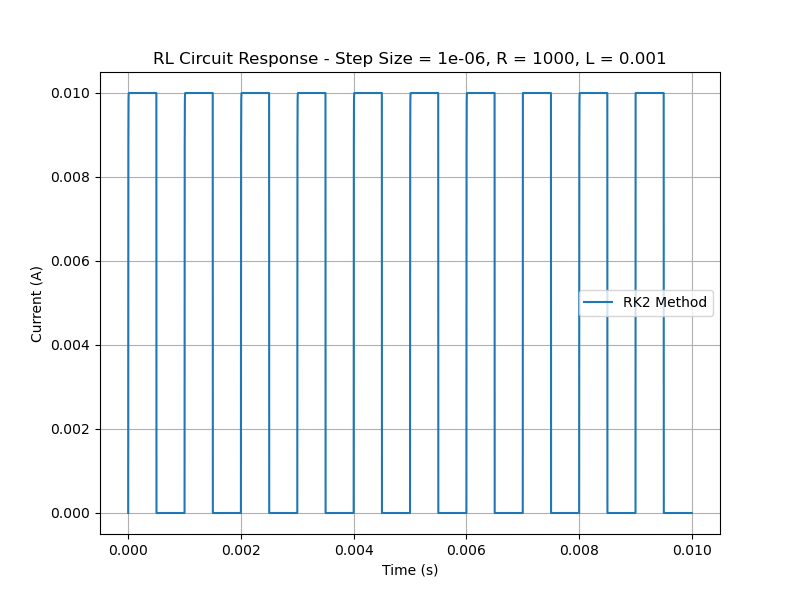
\includegraphics[ width=0.5\textwidth]{./figs/rk2_R1000_L0.001.png}}
\hspace{\fill}
{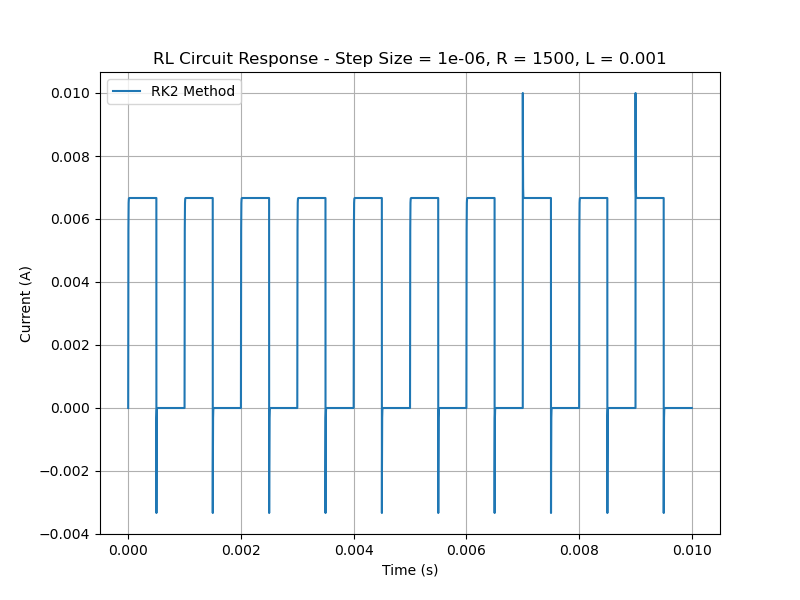
\includegraphics[ width=0.5\textwidth]{./figs/rk2_R1500_L0.001.png}}
\end{figure*}
\begin{figure*}[!htb]
{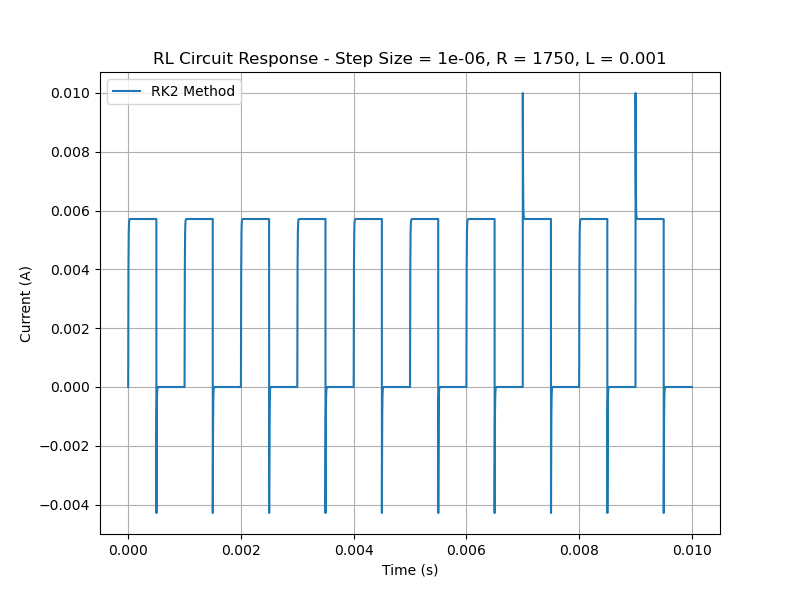
\includegraphics[ width=0.5\textwidth]{./figs/rk2_R1750_L0.001.png}}
\hspace{\fill}
{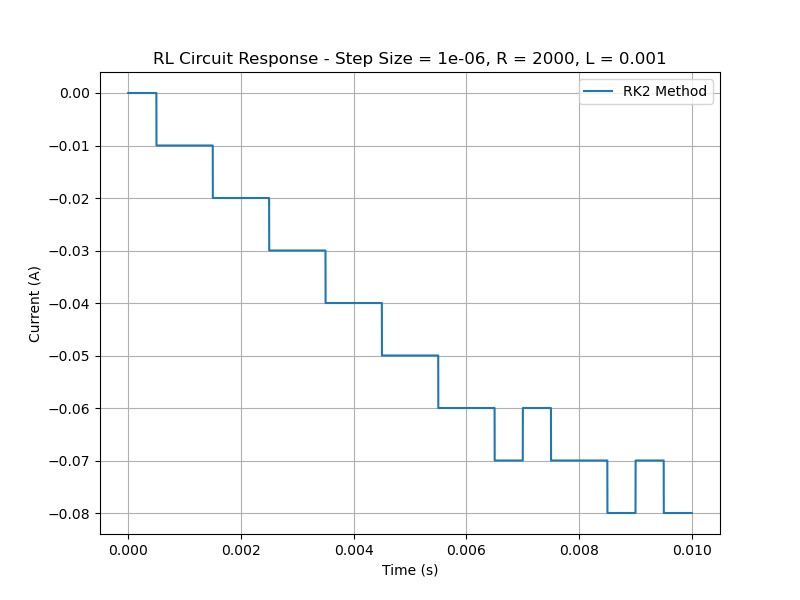
\includegraphics[ width=0.5\textwidth]{./figs/rk2_R2000_L0.001.png}}
\end{figure*}
\begin{figure*}[!htb]
{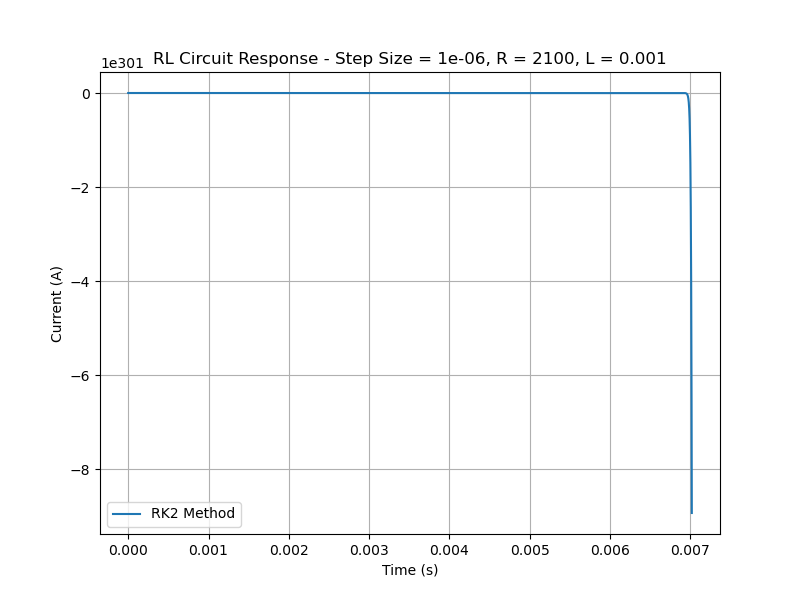
\includegraphics[ width=0.99\textwidth]{./figs/rk2_R2100_L0.001.png}}
\end{figure*}

The stability boundary for RK2 is the same as for Forward Euler in this case, both requiring $\frac{R}{L} < \frac{2}{h}$, despite RK2 being a higher-order method. The difference between the methods lies in their accuracy rather than their stability boundaries for this particular problem.

While both methods become unstable at the same theoretical boundary, RK2 typically shows better behavior near the stability limit due to its higher order of accuracy. This can be observed in the less severe oscillations at $R = 2000$ compared to the Forward Euler method. However, once the stability boundary is crossed at $R = 2100$, both methods exhibit catastrophic instability.

\subsection{RK4 Method}
The update equation for RK4 method is given by,
\begin{align*}
i_{n+1} &= i_n + \frac{h}{6}(k_1 + 2k_2 + 2k_3 + k_4)
\end{align*}

Where:
\begin{align*}
k_1 &= f(t_n, i_n)\\
k_2 &= f\left(t_n + \frac{h}{2}, i_n + \frac{h}{2}k_1\right)\\
k_3 &= f\left(t_n + \frac{h}{2}, i_n + \frac{h}{2}k_2\right)\\
k_4 &= f(t_n + h, i_n + hk_3)
\end{align*}

For our circuit equation with $f(t, i) = \frac{1}{L}(V_{in}(t) - iR)$, the growth factor for a linear system can be derived by applying RK4 to the test equation $i' = \lambda i$ where $\lambda = -\frac{R}{L}$.

Growth factor for RK4 is given by,
\begin{align*}
    1 + z + \frac{z^2}{2!} + \frac{z^3}{3!} + \frac{z^4}{4!}\\
    = 1 + z + \frac{z^2}{2} + \frac{z^3}{6} + \frac{z^4}{24}
\end{align*}
where $z = \lambda h = -\frac{R}{L}h$. \newline
This is a result of RK4 being derived from the taylor series expansion of the function $f\brak{i, t}$.\newline\newline
Let's denote $\frac{R}{L} = \alpha$. Therefore, the growth factor for RK4 is now given by,
\begin{align*}
G = 1 - \alpha h + \frac{(\alpha h)^2}{2} - \frac{(\alpha h)^3}{6} + \frac{(\alpha h)^4}{24}
\end{align*}

For the system to be stable,
\begin{align*}
    \abs{G} < 1\\
    \implies &\abs{1 - \alpha h + \frac{(\alpha h)^2}{2} - \frac{(\alpha h)^3}{6} + \frac{(\alpha h)^4}{24}} < 1
\end{align*}

Upon solving this, we get,
\begin{align*}
0 < \alpha h &< 2.785\\
\implies \frac{R}{L} &< \frac{2.785}{h}
\end{align*}

This is a less restrictive condition than the RK2 method, which required $\frac{R}{L} < \frac{2}{h}$. The larger stability region of RK4 allows for larger step sizes while maintaining numerical stability.

For the complete circuit equation including the input voltage terms, the full RK4 update would be,
\begin{align*}
i_{n+1} = G \cdot i_n + \text{terms involving } V_{in}
\end{align*}

\textbf{Local Truncation Error}: The local truncation error for RK4 is $O(h^5)$. This high-order accuracy comes from incorporating terms up to the fourth derivative in the Taylor series expansion.

\textbf{Global Truncation Error}: The global truncation error for RK4 is $O(h^4)$. This fourth-order accuracy makes it exceptionally efficient for smooth problems.

\textbf{Error Characteristics}:
\begin{itemize}
\item Fourth-order convergence (halving step size reduces error by factor of 16).
\item Remains stable at resistance values where lower-order methods fail.
\item Uses weighted average of four slope calculations to better capture the solution/response.
\end{itemize}

For the purpose of this analysis, we take $R = 1000, 1500, 1750, 2000, 2250, 2750, 2850$, $L = 0.001$ and step size $\brak{h} = 10^{-6}$.\newline
Stability is achieved when,
\begin{align*}
\frac{R}{L} &< \frac{2.785}{h}\\
\frac{R}{L} &< 2.785\times10^6\\
\implies R &< 2785
\end{align*}

\begin{figure*}[!htb]
{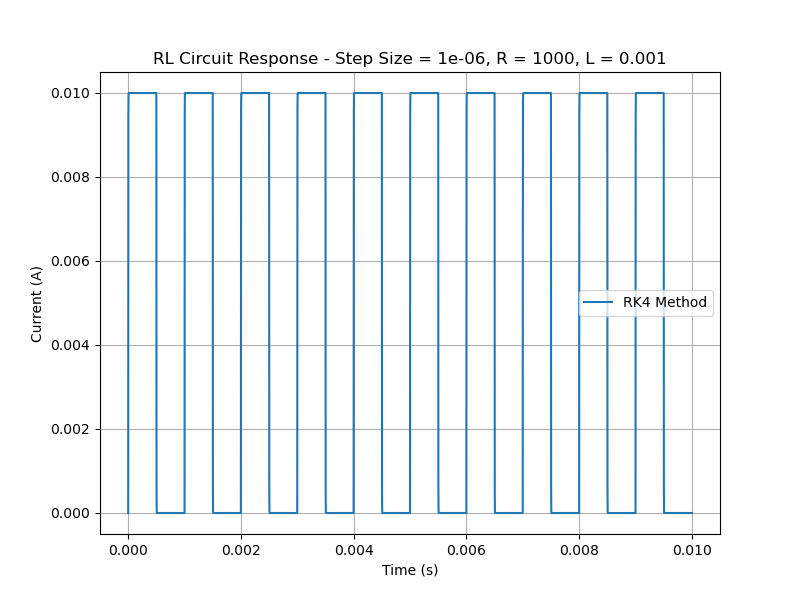
\includegraphics[ width=0.5\textwidth]{./figs/rk4_R1000_L0.001.png}}
\hspace{\fill}
{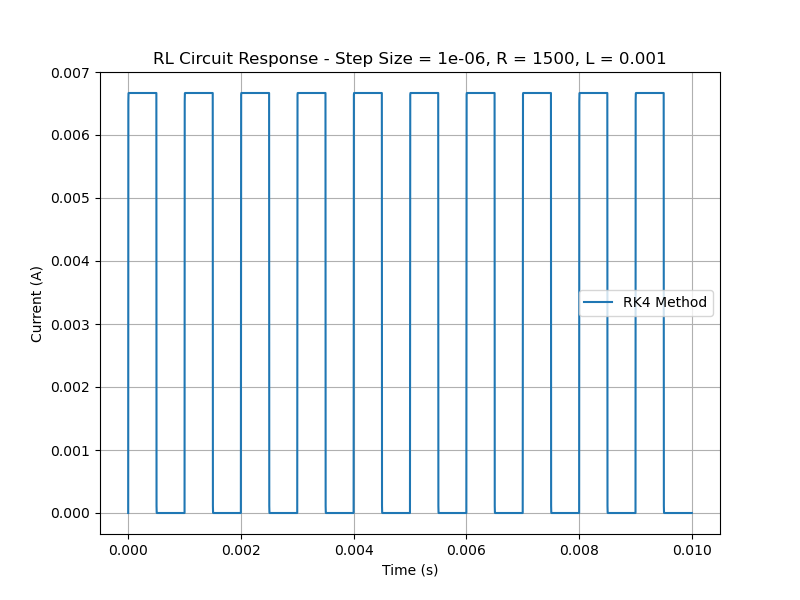
\includegraphics[ width=0.5\textwidth]{./figs/rk4_R1500_L0.001.png}}
\end{figure*}
\begin{figure*}[!htb]
{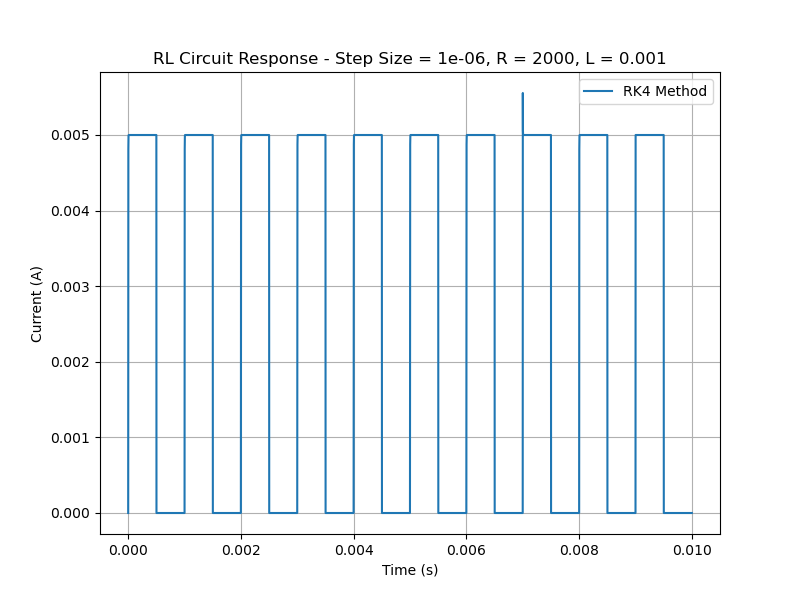
\includegraphics[ width=0.5\textwidth]{./figs/rk4_R2000_L0.001.png}}
\hspace{\fill}
{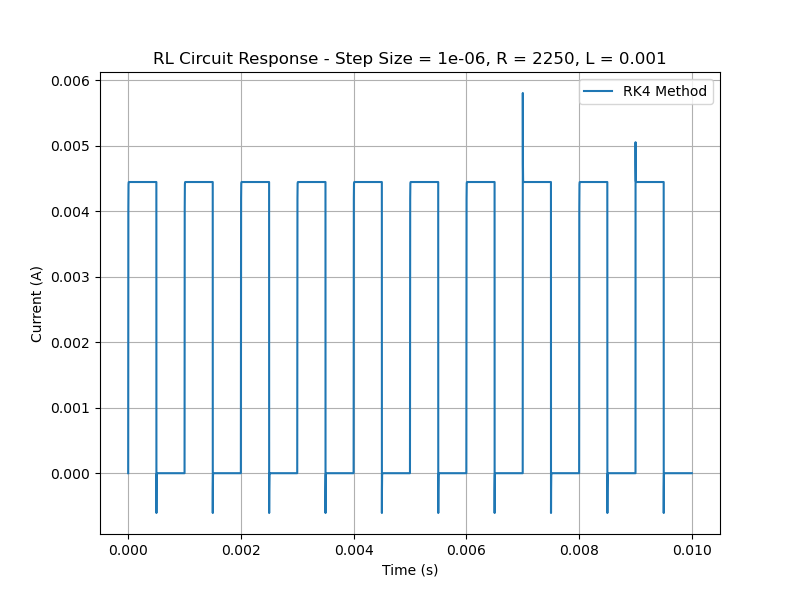
\includegraphics[ width=0.5\textwidth]{./figs/rk4_R2250_L0.001.png}}
\end{figure*}
\begin{figure*}[!htb]
{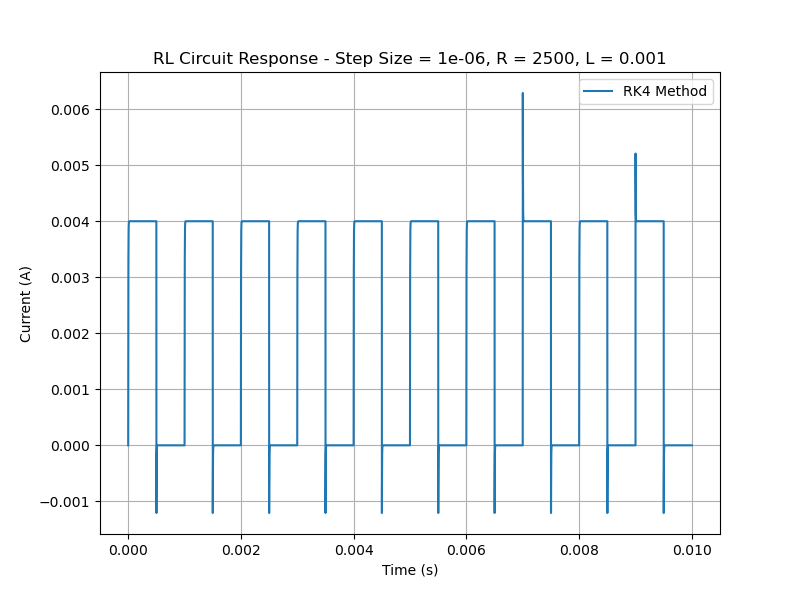
\includegraphics[ width=0.5\textwidth]{./figs/rk4_R2500_L0.001.png}}
\hspace{\fill}
{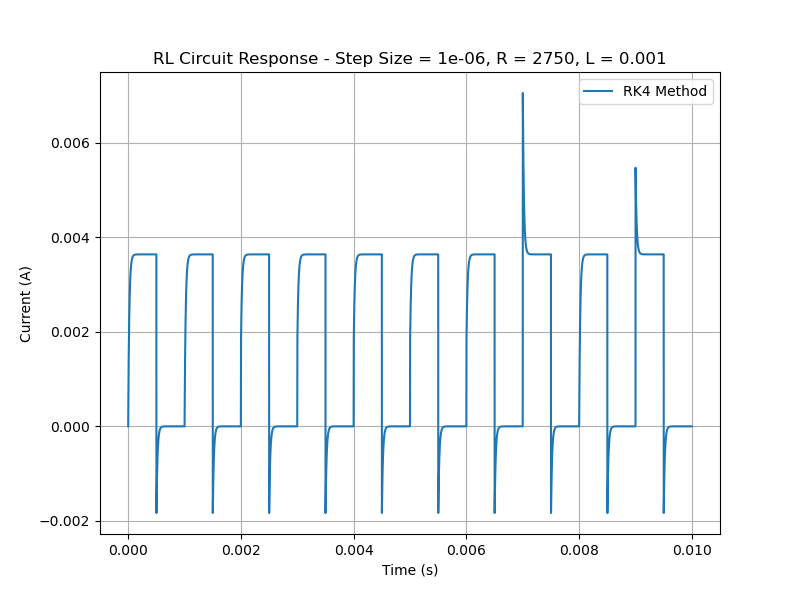
\includegraphics[ width=0.5\textwidth]{./figs/rk4_R2750_L0.001.png}}
\end{figure*}
\begin{figure*}[!htb]
{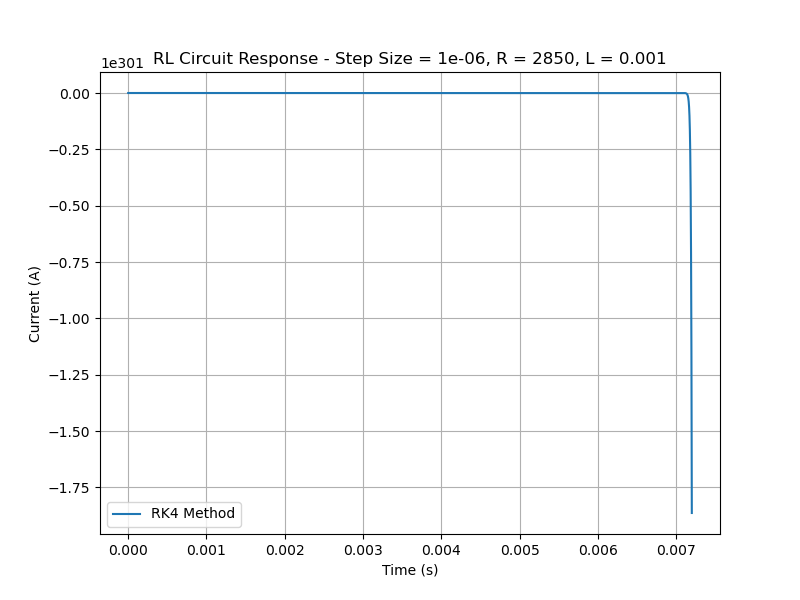
\includegraphics[ width=0.99\textwidth]{./figs/rk4_R2850_L0.001.png}}
\end{figure*}

The RK4 method demonstrates superior stability characteristics compared to both Forward Euler and RK2 methods. The stability boundary extends approximately 39\% further (from $R = 2000$ to $R = 2785$), allowing for more efficient simulation of stiffer systems without requiring smaller step sizes.
\newline

This improved stability, combined with RK4's fourth-order accuracy, makes it particularly well-suited for circuit simulations where both accuracy and efficiency are important. The ability to use larger step sizes while maintaining stability can significantly reduce computation time for complex circuit simulations, especially when dealing with components that introduce stiffness into the system.
\newline

However, it's worth noting that for extremely stiff systems (very high R/L ratios), even RK4 would require relatively small step sizes. In such cases, implicit methods like Backward Euler or the Trapezoidal method, which are unconditionally stable, would be more appropriate despite their lower order of accuracy.

\subsection{Trapezoidal Method}
The update equation for the trapezoidal method is given by,
\begin{align*}
i_{n+1} &= i_n + \frac{h}{2} \Big[ f(t_n, i_n) + f(t_{n+1}, i_{n+1}) \Big]
\end{align*}

For our circuit equation with $f(t, i) = \frac{1}{L}(V_{in}(t) - iR)$, we have
\begin{align*}
i_{n+1} &= i_n + \frac{h}{2} \Big[ \frac{1}{L}(V_{in}(t_n) - i_n R) + \frac{1}{L}(V_{in}(t_{n+1}) - i_{n+1} R) \Big] \\
i_{n+1} &= i_n + \frac{h}{2L} \Big[ V_{in}(t_n) - i_n R + V_{in}(t_{n+1}) - i_{n+1} R \Big]
\end{align*}

Rearranging to isolate $i_{n+1}$,
\begin{align*}
i_{n+1} + \frac{hR}{2L}i_{n+1} &= i_n + \frac{h}{2L} \Big[ V_{in}(t_n) - i_n R + V_{in}(t_{n+1}) \Big] \\
i_{n+1}\Big(1 + \frac{hR}{2L}\Big) &= i_n\Big(1 - \frac{hR}{2L}\Big) + \frac{h}{2L} \Big[ V_{in}(t_n) + V_{in}(t_{n+1}) \Big] \\
i_{n+1} &= i_n\brak{\frac{1 - \frac{hR}{2L}}{1 + \frac{hR}{2L}}} + \frac{h}{2L}\frac{1}{\brak{1 + \frac{hR}{2L}}} \Big[ V_{in}(t_n) + V_{in}(t_{n+1}) \Big]
\end{align*}

The growth factor for the trapezoidal method is therefore,
\begin{align*}
G = \frac{1 - \frac{hR}{2L}}{1 + \frac{hR}{2L}}
\end{align*}

Let $\alpha = \frac{R}{L}$. For stability, we need $|G| < 1$,
\begin{align*}
\left|\frac{1 - \frac{\alpha h}{2}}{1 + \frac{\alpha h}{2}}\right| &< 1\\
\implies -1 < \frac{1 - \frac{\alpha h}{2}}{1 + \frac{\alpha h}{2}} &< 1
\end{align*}

Since $\alpha > 0$ and $h > 0$, we have $1 + \frac{\alpha h}{2} > 0$.\newline
For the right inequality ($\frac{1 - \frac{\alpha h}{2}}{1 + \frac{\alpha h}{2}} < 1$):
\begin{align*}
\frac{1 - \frac{\alpha h}{2}}{1 + \frac{\alpha h}{2}} &< 1 \\
1 - \frac{\alpha h}{2} &< 1 + \frac{\alpha h}{2} \\
-\frac{\alpha h}{2} &< \frac{\alpha h}{2} \\
0 &< \alpha h
\end{align*}
Since $\alpha > 0$ and $h > 0$, this inequality is always satisfied.

For the left inequality ($-1 < \frac{1 - \frac{\alpha h}{2}}{1 + \frac{\alpha h}{2}}$):
\begin{align*}
-1 &< \frac{1 - \frac{\alpha h}{2}}{1 + \frac{\alpha h}{2}} \\
-\left(1 + \frac{\alpha h}{2}\right) &< 1 - \frac{\alpha h}{2} \\
-1 - \frac{\alpha h}{2} &< 1 - \frac{\alpha h}{2} \\
-1 &< 1
\end{align*}
This is always true, so the trapezoidal method is unconditionally stable. This is consistent with the fact that the trapezoidal method is A-stable, meaning its region of absolute stability includes the entire left half-plane.

\textbf{Local Truncation Error}: The local truncation error for the Trapezoidal method is $O(h^3)$, comparable to RK2 despite being an implicit method.

\textbf{Global Truncation Error}: The global truncation error for the Trapezoidal method is $O(h^2)$, providing second-order accuracy.

\textbf{Error Characteristics}:
\begin{itemize}
\item Second-order convergence.
\item Maintains accuracy (to an extent) even at extreme resistance values ($R = 10000$).
\end{itemize}
For the purpose of this analysis, we take $R = 1000, 1500, 2000, 2500, 5000, 10000$, $L = 0.001$ and step size $\brak{h} = 10^{-6}$.

\begin{figure*}[!htb]
{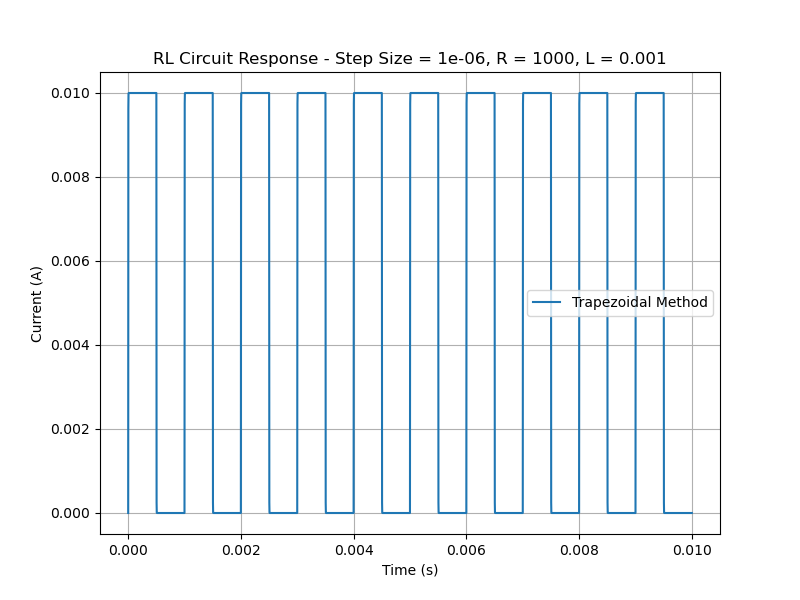
\includegraphics[ width=0.5\textwidth]{./figs/trapezoidal_R1000_L0.001.png}}
\hspace{\fill}
{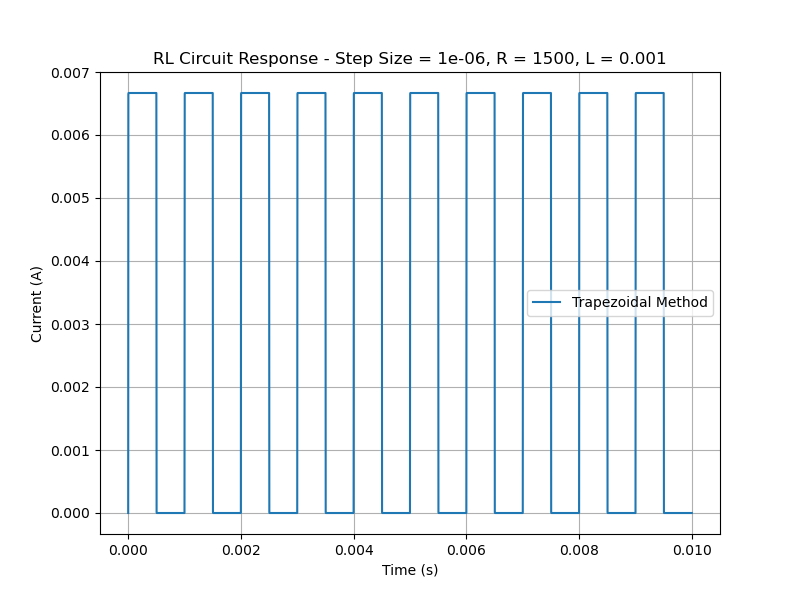
\includegraphics[ width=0.5\textwidth]{./figs/trapezoidal_R1500_L0.001.png}}
\end{figure*}
\begin{figure*}[!htb]
{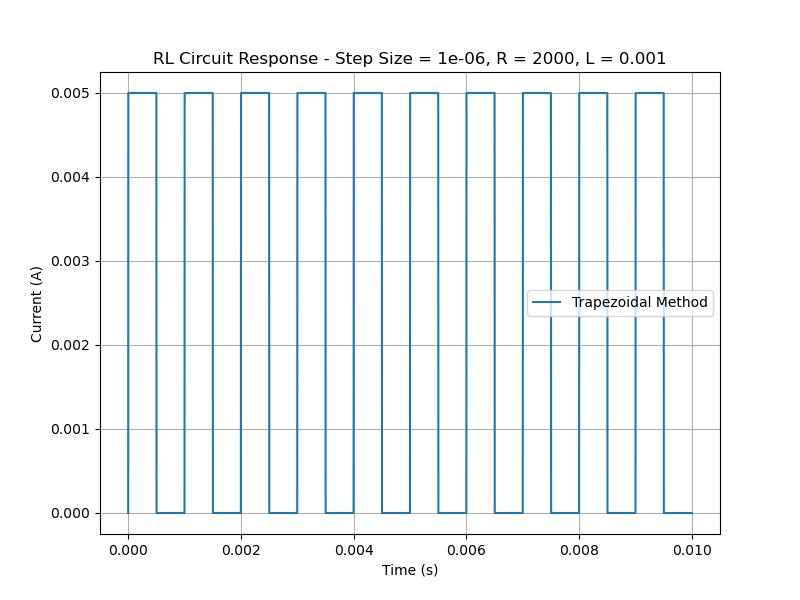
\includegraphics[ width=0.5\textwidth]{./figs/trapezoidal_R2000_L0.001.png}}
\hspace{\fill}
{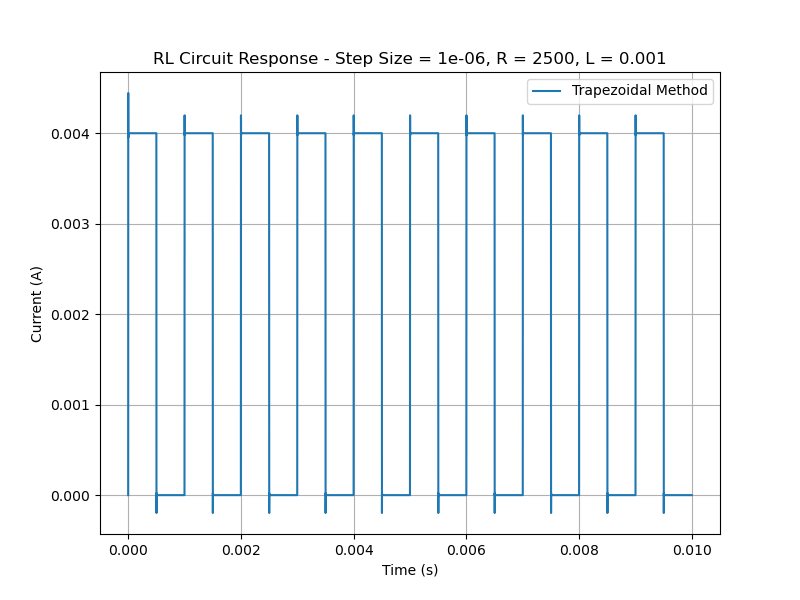
\includegraphics[ width=0.5\textwidth]{./figs/trapezoidal_R2500_L0.001.png}}
\end{figure*}
\begin{figure*}[!htb]
{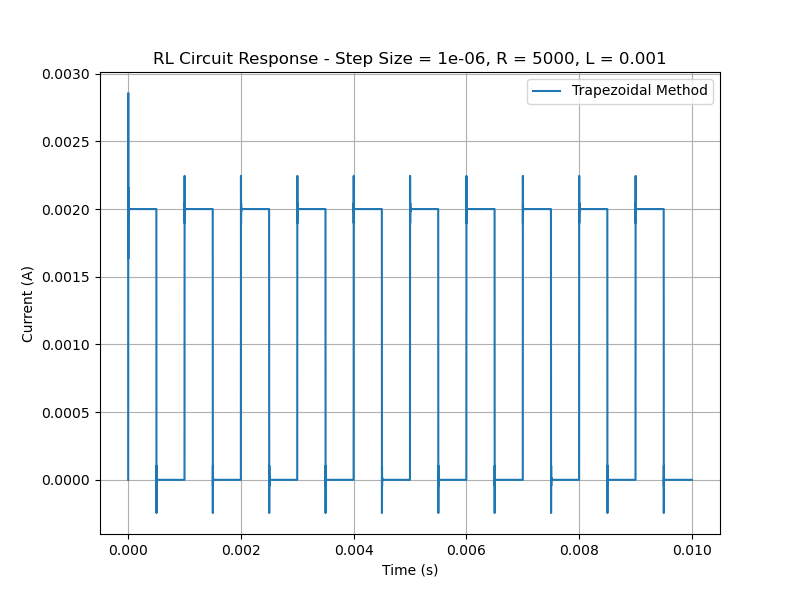
\includegraphics[ width=0.5\textwidth]{./figs/trapezoidal_R5000_L0.001.png}}
\hspace{\fill}
{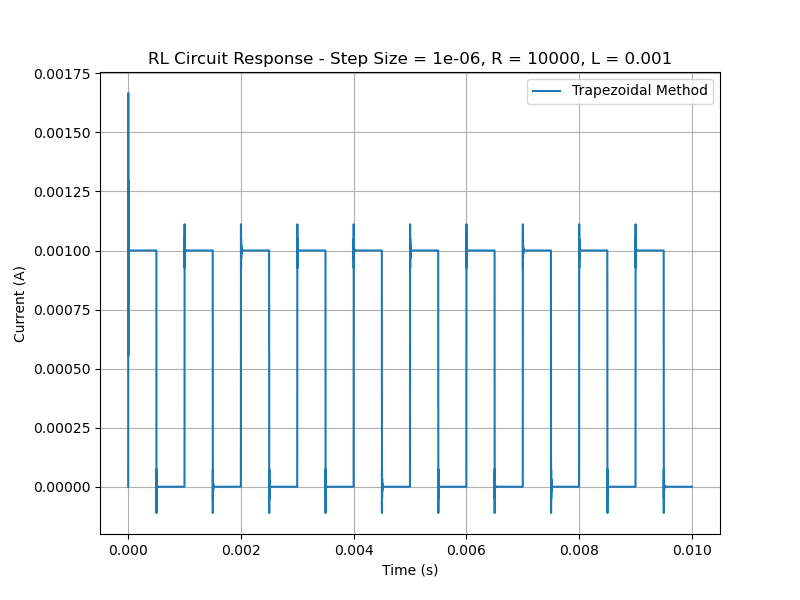
\includegraphics[ width=0.5\textwidth]{./figs/trapezoidal_R10000_L0.001.png}}
\end{figure*}

The trapezoidal method shows extreme stability across all resistance values tested. Unlike the explicit methods (Forward Euler, RK2, and RK4) which become unstable when $R$ exceeds their respective stability limits, the trapezoidal method remains stable even at $R = 10000$, which is 5 times higher than the stability limit of Forward Euler and RK2, and approximately 4 times higher than the stability limit of RK4.
\newline\newline

This unconditional stability makes the trapezoidal method particularly valuable for circuit simulations involving components with widely varying time constants or when the circuit parameters might change during operation. The method allows the use of reasonably large step sizes regardless of the stiffness of the system, potentially leading to significant computational savings.
\newline\newline

The only potential drawback of the trapezoidal method compared to explicit methods is the need to solve an implicit equation at each step, but for linear circuits like the one considered here, this can be done efficiently through direct computation rather than requiring iterative methods such as Newton Raphson Method.

\subsection{Backward Euler Method}
The update equation for the backward Euler method is given by,
\begin{align*}
i_{n+1} &= i_n + h f(t_{n+1}, i_{n+1})
\end{align*}

For our circuit equation with $f(t, i) = \frac{1}{L}(V_{in}(t) - iR)$, we have
\begin{align*}
i_{n+1} &= i_n + \frac{h}{L}(V_{in}(t_{n+1}) - i_{n+1}R) \\
i_{n+1} &= i_n + \frac{h}{L}V_{in}(t_{n+1}) - \frac{hR}{L}i_{n+1}\\
i_{n+1} + \frac{hR}{L}i_{n+1} &= i_n + \frac{h}{L}V_{in}(t_{n+1}) \\
i_{n+1}\left(1 + \frac{hR}{L}\right) &= i_n + \frac{h}{L}V_{in}(t_{n+1}) \\
i_{n+1} &= \frac{i_n + \frac{h}{L}V_{in}(t_{n+1})}{1 + \frac{hR}{L}} \\
i_{n+1} &= \brak{\frac{1}{1 + \frac{hR}{L}}}i_n + \brak{\frac{\frac{h}{L}}{1 + \frac{hR}{L}}}V_{in}(t_{n+1})
\end{align*}

So the growth factor for the backward Euler method is given by,
\begin{align*}
G = \frac{1}{1 + \frac{hR}{L}}
\end{align*}

Let $\alpha = \frac{R}{L}$. For stability, we need $|G| < 1$,
\begin{align*}
\left|\frac{1}{1 + \alpha h}\right| &< 1
\end{align*}

Since $\alpha > 0$ and $h > 0$, we have $1 + \alpha h > 1 > 0$. Therefore,
\begin{align*}
0 < \frac{1}{1 + \alpha h} &< 1\\
\implies 0 < G &< 1\\
\implies \abs{G} &< 1
\end{align*}
This inequality is always satisfied for positive values of $\alpha$ and $h$.

Therefore, the backward Euler method is unconditionally stable for this circuit problem, meaning there is no restriction on the step size $h$ for stability. This is consistent with the fact that the backward Euler method is A-stable, making it particularly suitable for stiff differential equations.

\textbf{Local Truncation Error}: The local truncation error for Backward Euler is $O(h^2)$, identical to Forward Euler despite being an implicit method.

\textbf{Global Truncation Error}: The global truncation error for Backward Euler is $O(h)$, making it first-order accurate like Forward Euler.

\textbf{Error Characteristics}:
\begin{itemize}
\item First-order convergence.
\item Introduces artificial numerical damping for very stiff systems, which turns out to be beneficial in this case.
\item Particularly valuable during initial transients or for extremely stiff components.
\item Maintains smooth solutions even at $R = 10000$ where explicit methods fail.
\end{itemize}
The backward Euler method tends to introduce numerical damping, which can be beneficial for suppressing high-frequency oscillations that might arise from numerical errors, but may also artificially dampen physical oscillations in the circuit.

For the purpose of this analysis, we take $R = 1000, 1500, 2000, 2500, 5000, 10000$, $L = 0.001$ and step size $\brak{h} = 10^{-6}$.\newline

The plots confirm the unconditional stability of the backward Euler method. Even with extremely high resistance values such as $R = 10000$ (which would cause severe instability in explicit methods), the backward Euler method maintains stability. This demonstrates the significant advantage of implicit methods for stiff systems.

\begin{figure*}[!htb]
{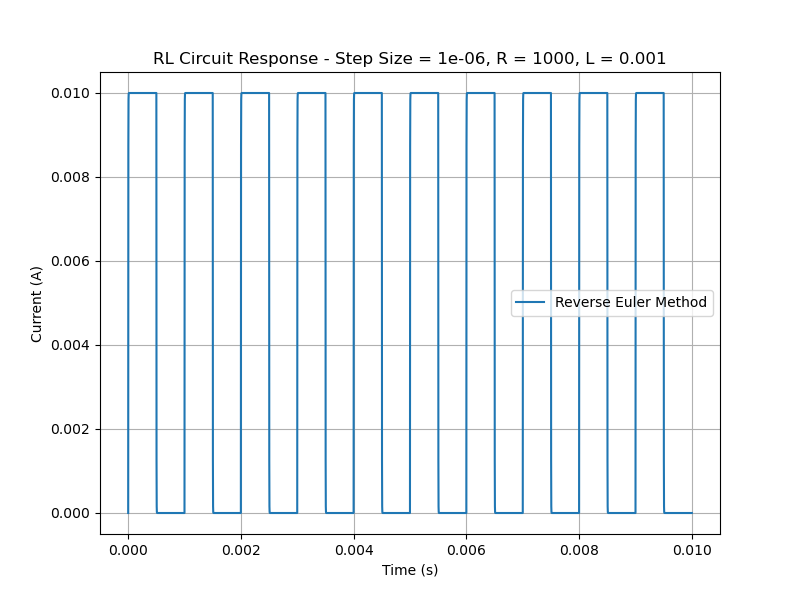
\includegraphics[ width=0.5\textwidth]{./figs/reverseEuler_R1000_L0.001.png}}
\hspace{\fill}
{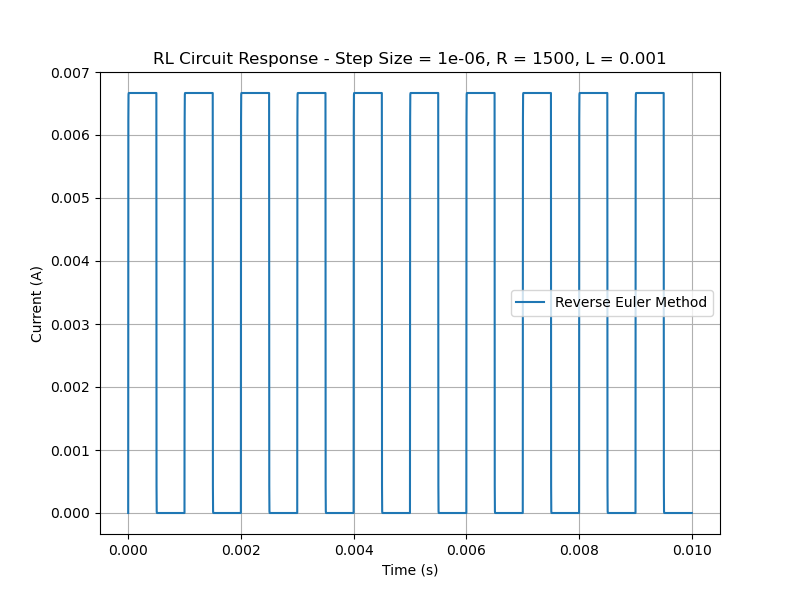
\includegraphics[ width=0.5\textwidth]{./figs/reverseEuler_R1500_L0.001.png}}
\end{figure*}
\begin{figure*}[!htb]
{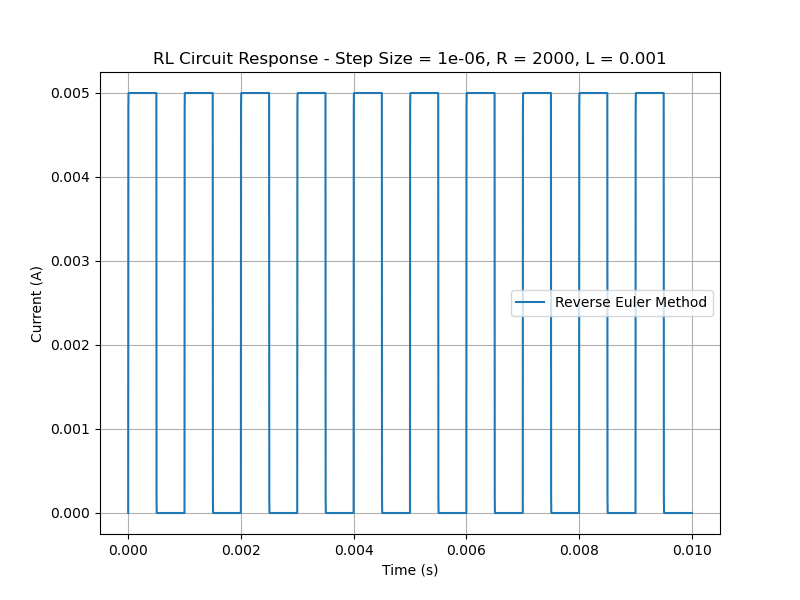
\includegraphics[ width=0.5\textwidth]{./figs/reverseEuler_R2000_L0.001.png}}
\hspace{\fill}
{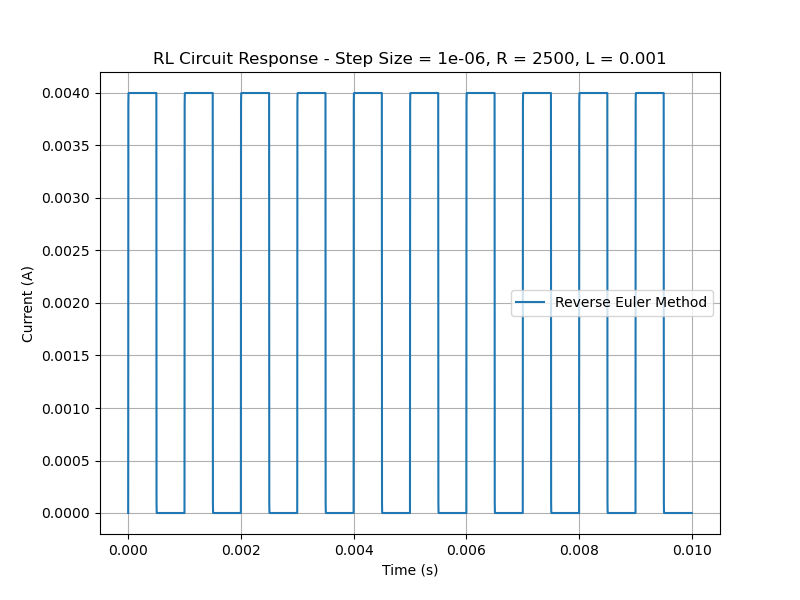
\includegraphics[ width=0.5\textwidth]{./figs/reverseEuler_R2500_L0.001.png}}
\end{figure*}
\begin{figure*}[!htb]
{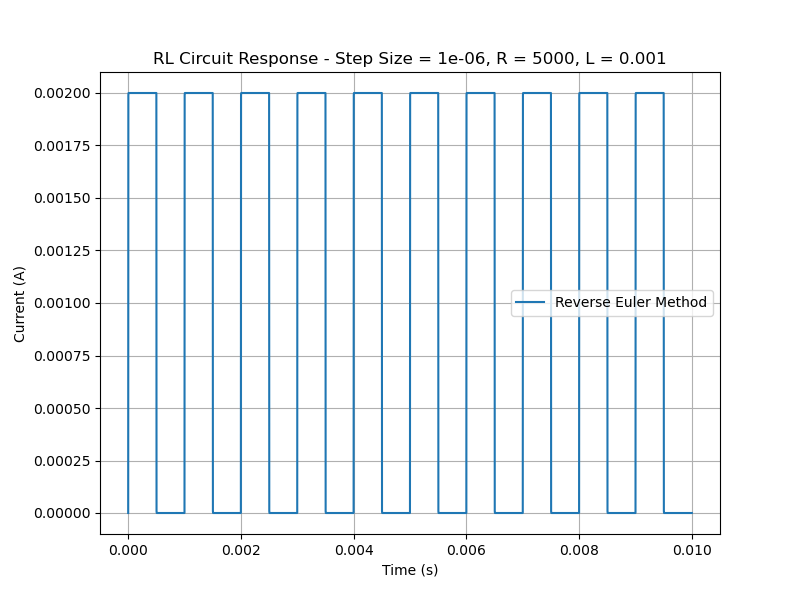
\includegraphics[ width=0.5\textwidth]{./figs/reverseEuler_R5000_L0.001.png}}
\hspace{\fill}
{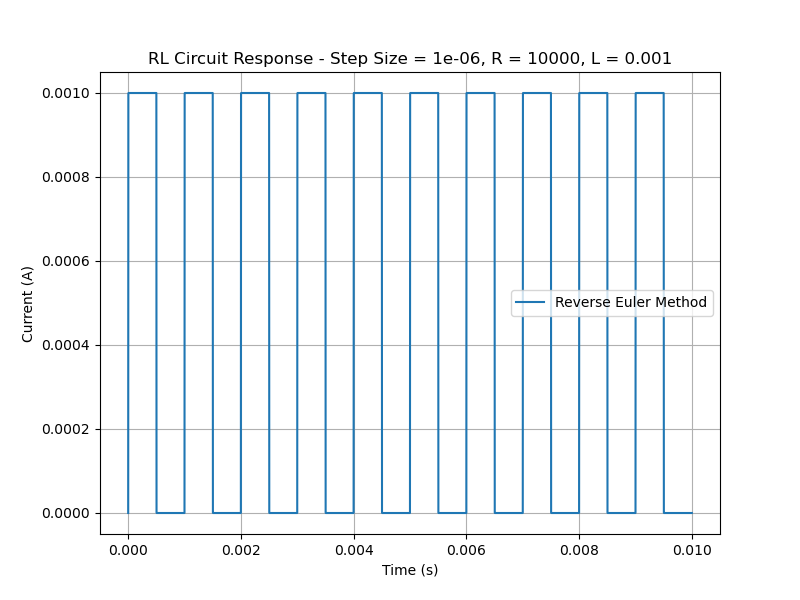
\includegraphics[ width=0.5\textwidth]{./figs/reverseEuler_R10000_L0.001.png}}
\end{figure*}

The backward Euler method is first-order accurate, compared to the second-order accuracy of the trapezoidal method. This means that for the same step size, the backward Euler method generally produces less accurate results. However, its strong stability properties, particularly for very stiff problems, can make it preferable in certain situations where stability is more critical than accuracy.
\newline\newline

Like the trapezoidal method, the backward Euler method requires solving an implicit equation at each step. For linear circuits like the one considered here, this can be done efficiently through direct computation. For nonlinear circuits, the strong stability of backward Euler can sometimes make it easier to solve the implicit equations compared to other methods.
\newline\newline

The backward Euler method is particularly valuable in circuit simulations during the initial transient phase or when dealing with components that introduce extreme stiffness into the system, where its robust stability characteristics outweigh its lower order of accuracy.

\end{document}
